\begin{appendices}

  \section{Data Protection \& Consent Form}
  \label{append:consent}

  \subsection*{Information about data protection and declaration of consent}

  Dear participant,

  thank you for your interest in participating in this study on ”Playful Experiences in the Onboarding Process of Software Development Projects”. This study takes place as a part of my master thesis on “Onboarding in Software Development Projects as a Space of Play”. The thesis is written as a part of the new Joint Master "Human-Computer Interaction" of the FH Salzburg and the University of Salzburg. In order to use your personal data, we would need your written declaration of consent. Please, carefully read the following information.

  \subsubsection*{General Study Information}

  The goal of this study is to research how software developers experience playful approaches on the onboarding process into new projects. The results of this study are going to contribute to the research body of both the software development field but also the field of “Play”. From the study results conclusions are going to be drawn about: The openness towards playful experiences in the software development field, possible hurdles on implementing such experiences, the general attitude of developers towards play in the field and the selection of what information to include in onboarding processes.

  \subsubsection*{Overall Study Procedure}

  The participant will take part in a hybrid-study setting. Part of the study consists of going through an interactive visualization of an open-source software project and revealing parts of information within some parts of the project. The other part of the study consists of questions on the visualization and general questions on the intersection of Play and software development. The study can be accessed online and can be finished online without additional work on the participants side. Overall the procedure should take between 15 and 25 minutes.

  \subsubsection*{Rights}

  The participation in this study is voluntary. You may withdraw or stop your participation at any time without incurring any consequences. Moreover, you can request information about the processed personal data at any time, even after the termination of the study (for further information see also Confidentiality and data processing). If you have any questions please contact the study leader.

  \subsubsection*{Risks}

  You do not incur any risks by participating in this study. If you feel uncomfortable during the study you can cancel at any time without giving reasons and without incurring any consequences.

  \subsubsection*{Confidentiality and Data Processing}

  Your data will only be processed within the aforementioned project if you give your written consent. The data is going to be processed via the Firebase platform (https://firebase.google.com/) on european servers. For additional information on their privacy and data protection guidelines visit their documentation at https://policies.google.com/u/0/privacy. The following data is going to be processed within the study:

  \begin{itemize}
    \item{Demographic Information (Name, Age, Professional Background, Years of Experience, Gender)}
    \item{Your actions within the visualization (Timestamps of Clicks and Mouse moves together with the timestamps of certain events)}
    \item{Your answers to the questions that are part of the study}
  \end{itemize}

  After the end of the study, the data is going to be exported from Firebase and the underlying app instance is going to be deleted. This data is going to be kept strictly confidential and is not going to be passed on to further third parties. The data is going to be analyzed and then used within my master thesis. If you only want to be mentioned anonymously in my thesis please indicate so at the bottom. If you are doing that your name and age are going to be hidden in my thesis and your data is only going to be connected to a random ID.

  \subsubsection*{Renumeration}

  You will not receive an expense allowance for participation.

  \subsubsection*{Consent}

  I have carefully read and understood the declaration of consent. Any additional questions were answered to my satisfaction. My participation is voluntary, and I know that I can withdraw at any time, even without giving reasons, without incurring any disadvantages. By clicking on “Agree” below I agree to the processing of my personal data collected for this study and I am willing to participate.

  \subsubsection*{Anonimity}

  I want to participate anonymously (the data is not going to be connected to your name)

  \section{Probe Development Process}
  \label{append:probe-design}

  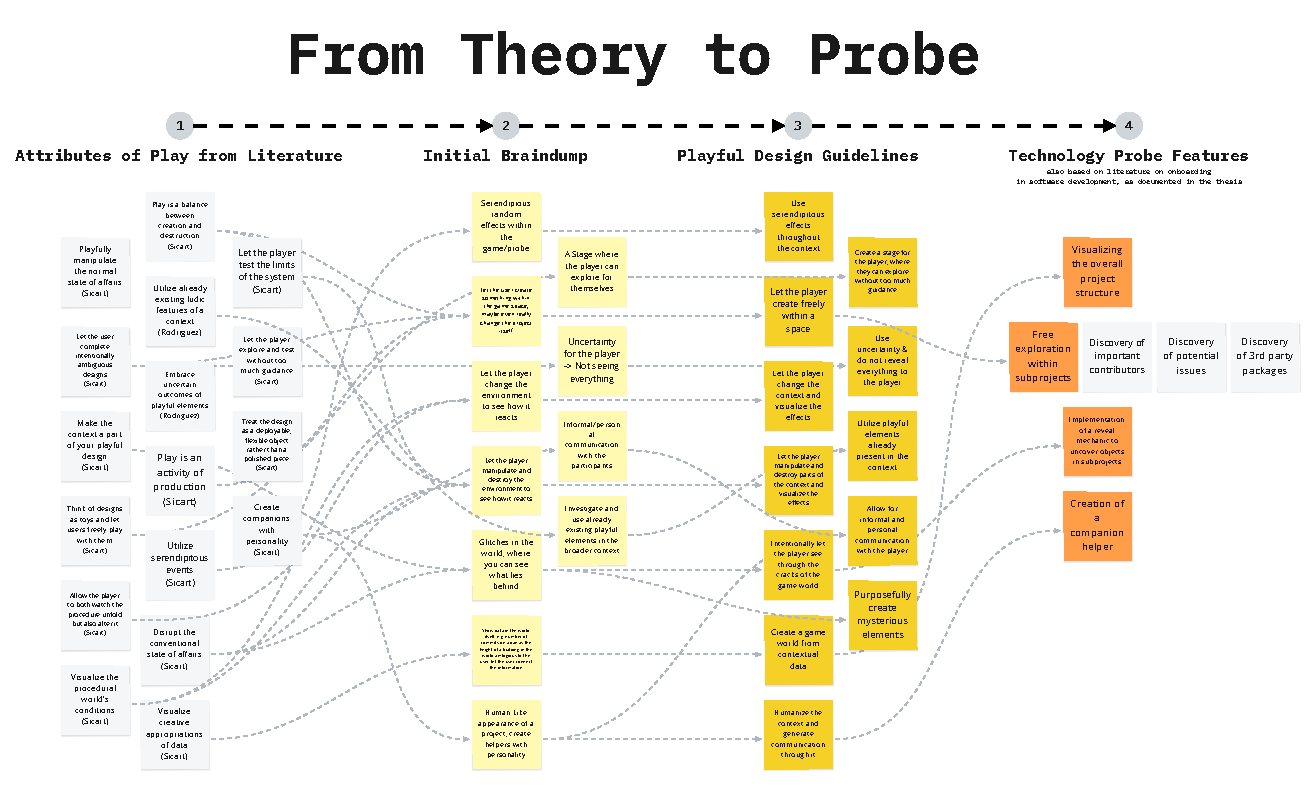
\includegraphics[angle=90,width=0.95\textwidth]{probedesign.pdf}

  \section{Probe Execution Process}
  \label{append:probe-exec}

  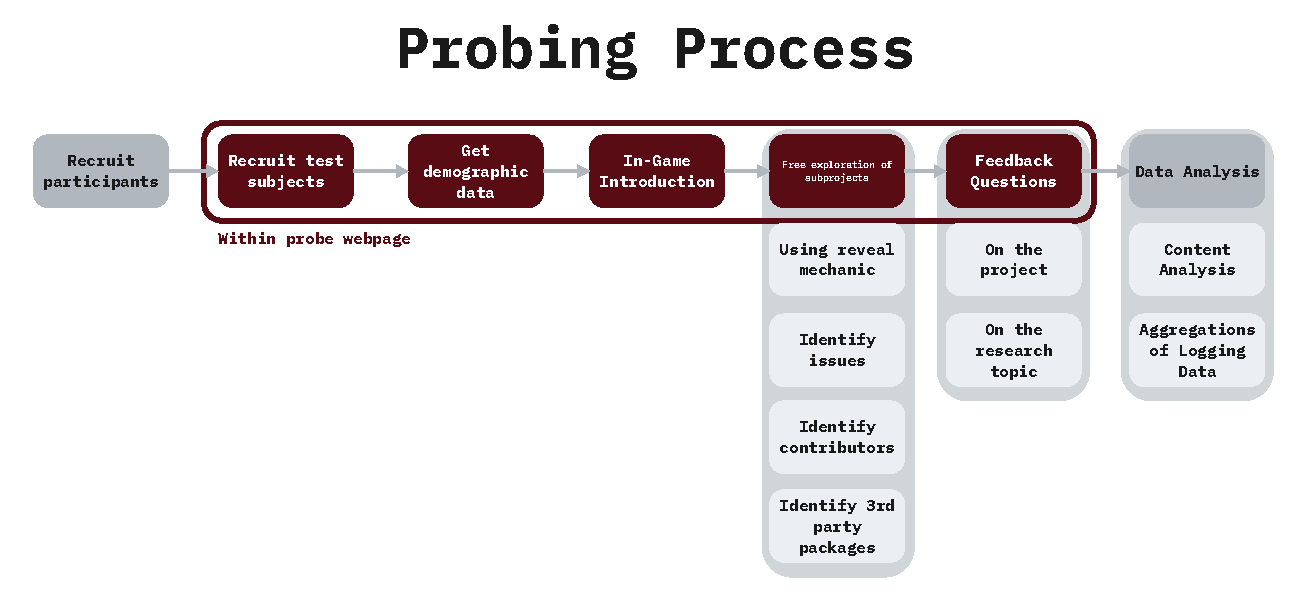
\includegraphics[angle=90,width=0.75\textwidth]{probeprocess.pdf}

  \section{Probe Information Message Types}
  \label{append:probe-types}

  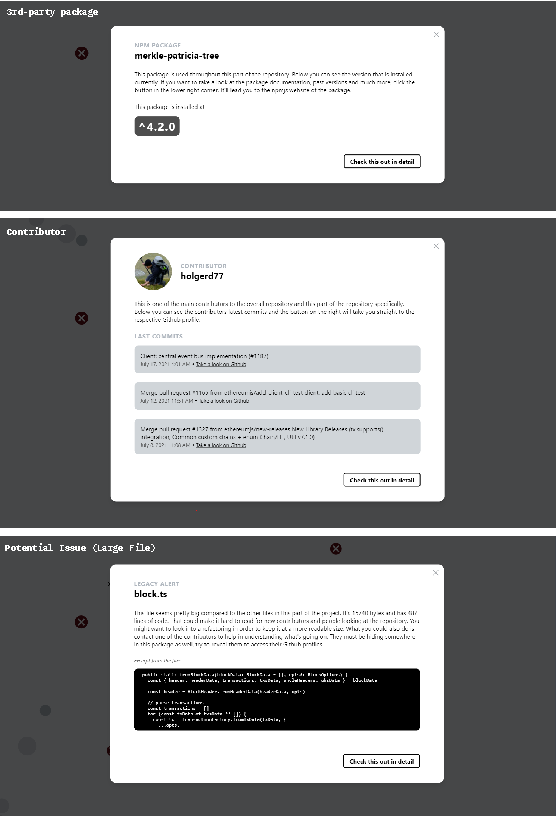
\includegraphics[width=\textwidth]{proberevealables.pdf}

  \section{Probe Data Collection -- Questions}
  \label{append:collect}

  \subsection*{Demographic Information}

  Text Input: \textbf{Your Name}

  Number Input: \textbf{Your Age}

  Text Input: \textbf{Your Professional Background}

  Select Input: \textbf{Your Professional Experience} (Options: 0-1 years, 1-3 years, 3-5 years, 5-10years)

  \subsection*{Questions on the underlying project}

  1) Do you remember any of the contributors of this project? Please name those that you remember below

  2) What were the two largest packages of this monorepo (not the npm packages, but the ones the monorepo is made out of)?

  3) Which of the projects "sub"-packages were used most throughout the other subpackages?

  4) Any npm packages you've revealed in this project, that you can think of? Did you take a look at their respective websites?

  5) Have you taken a look at any of the files that were potentially "legacy" files? If yes, did you agree on them being "refactor-worthy" or do you think they were fine as-is?

  \subsection*{Questions on the research topic}

  1) Would you say, that you have discovered something interesting about the underlying project from going through this interactive visualization? If yes, what? If no, what was missing or what would you have liked to see?

  2) What was your overall experience going through this visualization? What did you like or did not like?

  3) How did you experience the companion (lower right)? Was it helpful, annoying or did you not really interact with it at all?

  4) Could you imagine yourself using some kind of interactive visualization or something similar on different projects to learn about them? If so, on which projects would you want to try it out? If not, what would you prefer instead to make yourself familiar with new projects?

  5) How do you usually approach the onboarding onto new projects? To whom do you talk to, what applications do you use, how do you navigate through code?

  6) Do you work on Open Source Projects? If you are a contributor of one, how do you try to make it easy for new collaborators to work on these projects? If not, how do you approach collaborating for yourself?

  7) Do you have any additional ideas on how playful elements or game mechanics could be used within the onboarding phase of software development projects?

  8) What is your general stance on using games/game mechanics or playful elements within software development? Do you see a difference of using such mechanics in open source software vs. in a work environment?

  9) Do you have any additional ideas on how playful elements or game mechanics could be used within the onboarding phase of software development projects? Any elements from games you play that you think could be reused when making yourself familiar with new projects?

  10) Anything else you want to mention?

  \newpage
  \section{Probe Data Collection -- Logging}
  \label{append:collect-log}

  \subsection*{Logging Single Event Format}

  \begin{itemize}
    \item{\textbf{message}: Additional information depending on the event type}
    \item{\textbf{timestamp}: The unix timestamp at which the event occured}
    \item{\textbf{type}: The type of interaction according to the event codes below}
  \end{itemize}

  \subsection*{Logging Event Codes with their respective interactions}

  \begin{table}[h]
    \begin{tabularx}{\textwidth}{|X|X|X|}
      \hline
      \textbf{Event Code} & \textbf{Interaction}   \\ \hline \hline
      CC                  & Click on companion     \\ \hline
      OC                  & Overview click         \\ \hline
      RC                  & Reveal click           \\ \hline
      LI                  & Legacy identified      \\ \hline
      LR                  & Legacy revealed        \\ \hline
      PI                  & Package identified     \\ \hline
      PR                  & Package revealed       \\ \hline
      NI                  & Contributor identified \\ \hline
      NR                  & Contributor revealed   \\ \hline
      SF                  & Subproject finished    \\ \hline
      GF                  & Game finished          \\ \hline
    \end{tabularx}
  \end{table}

  \newpage

  \section{Technology Probe Scenes}
  \label{append:probe-steps}

  \subsection*{Step 1: Introduction}

  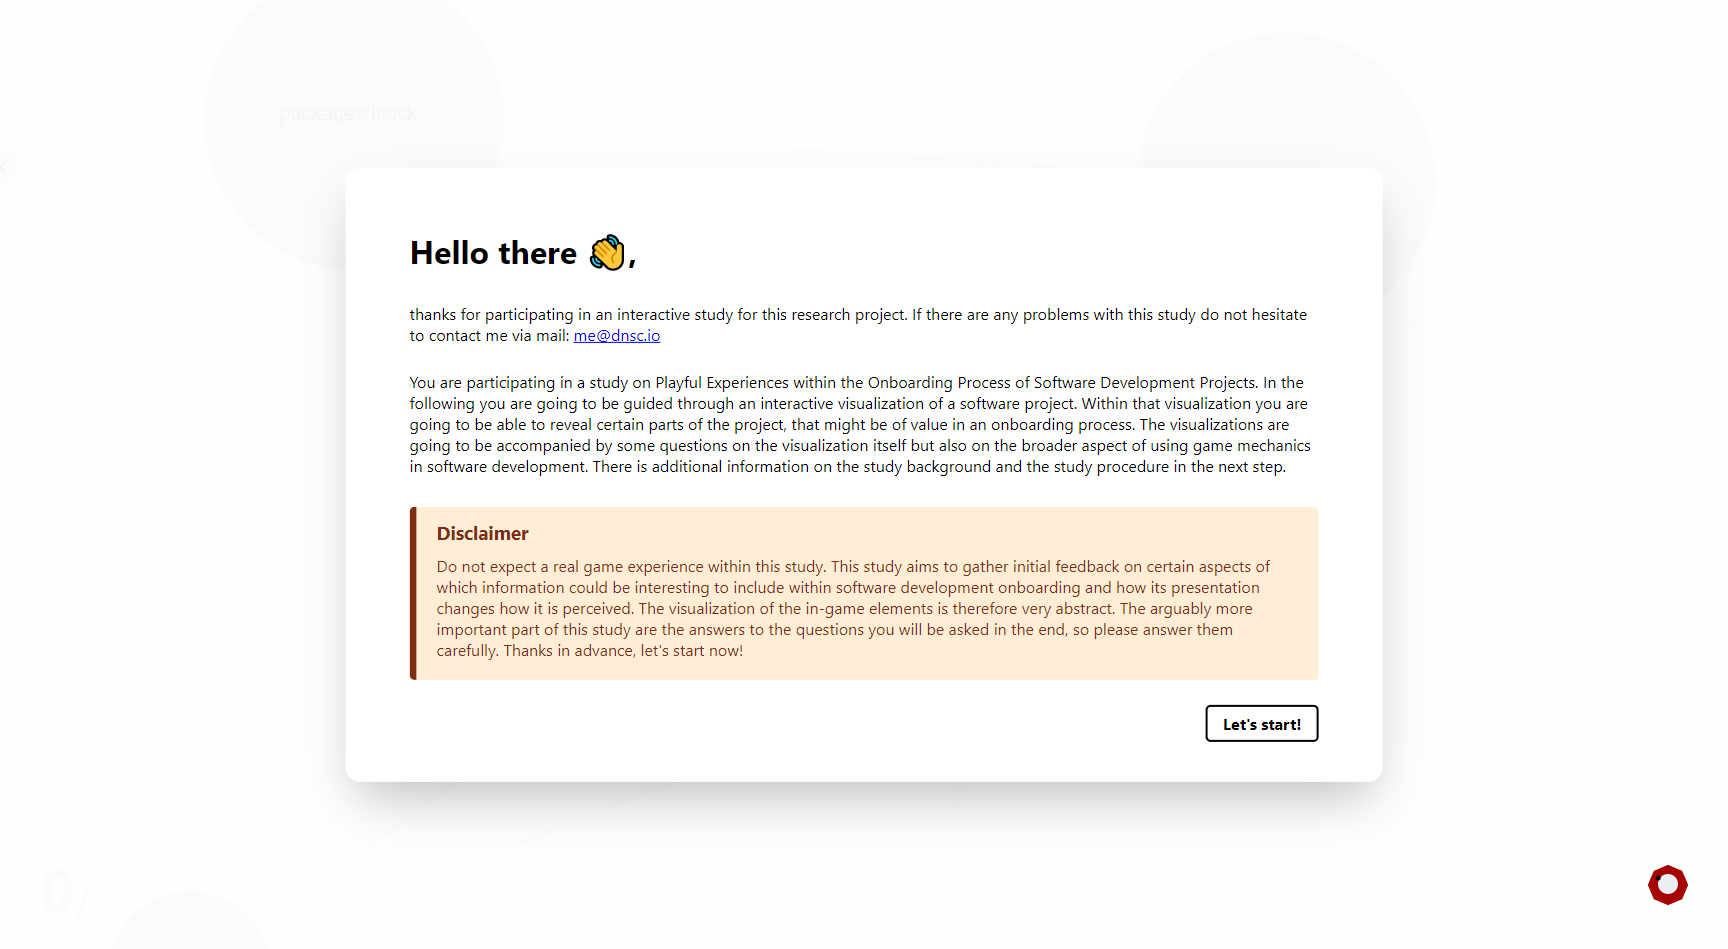
\includegraphics[width=\textwidth]{probesteps/step1.png}

  \subsection*{Step 2: Consent \& Data Protection}

  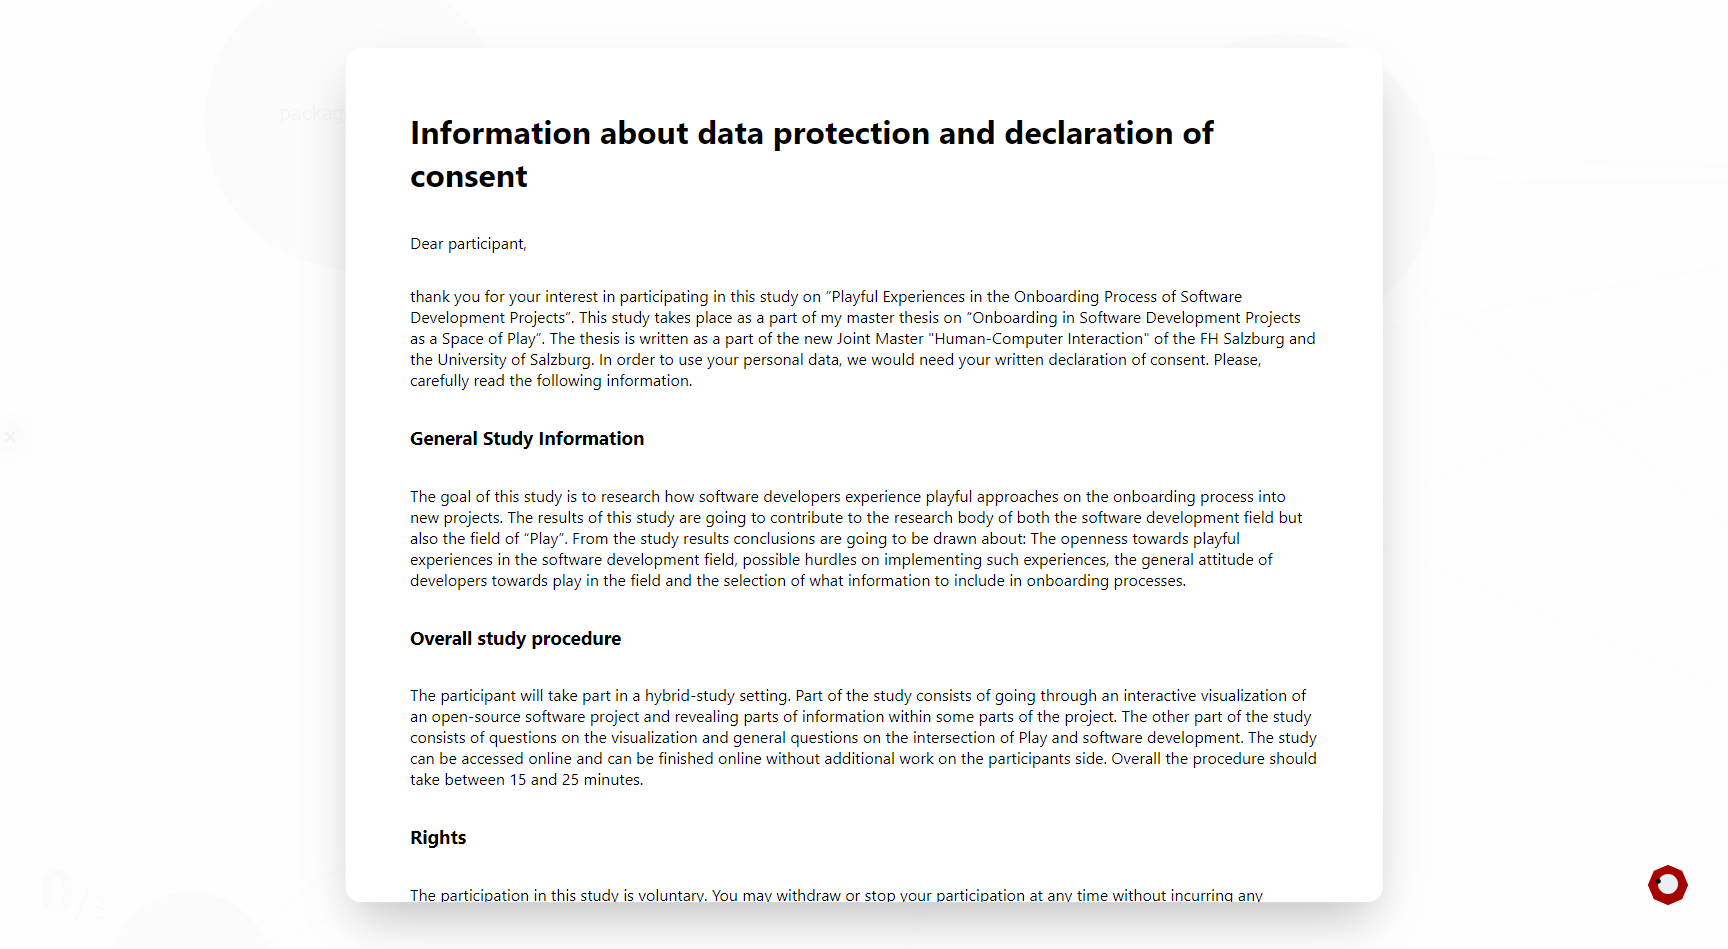
\includegraphics[width=\textwidth]{probesteps/step2.png}

  \subsection*{Step 3: Demographic Questions}

  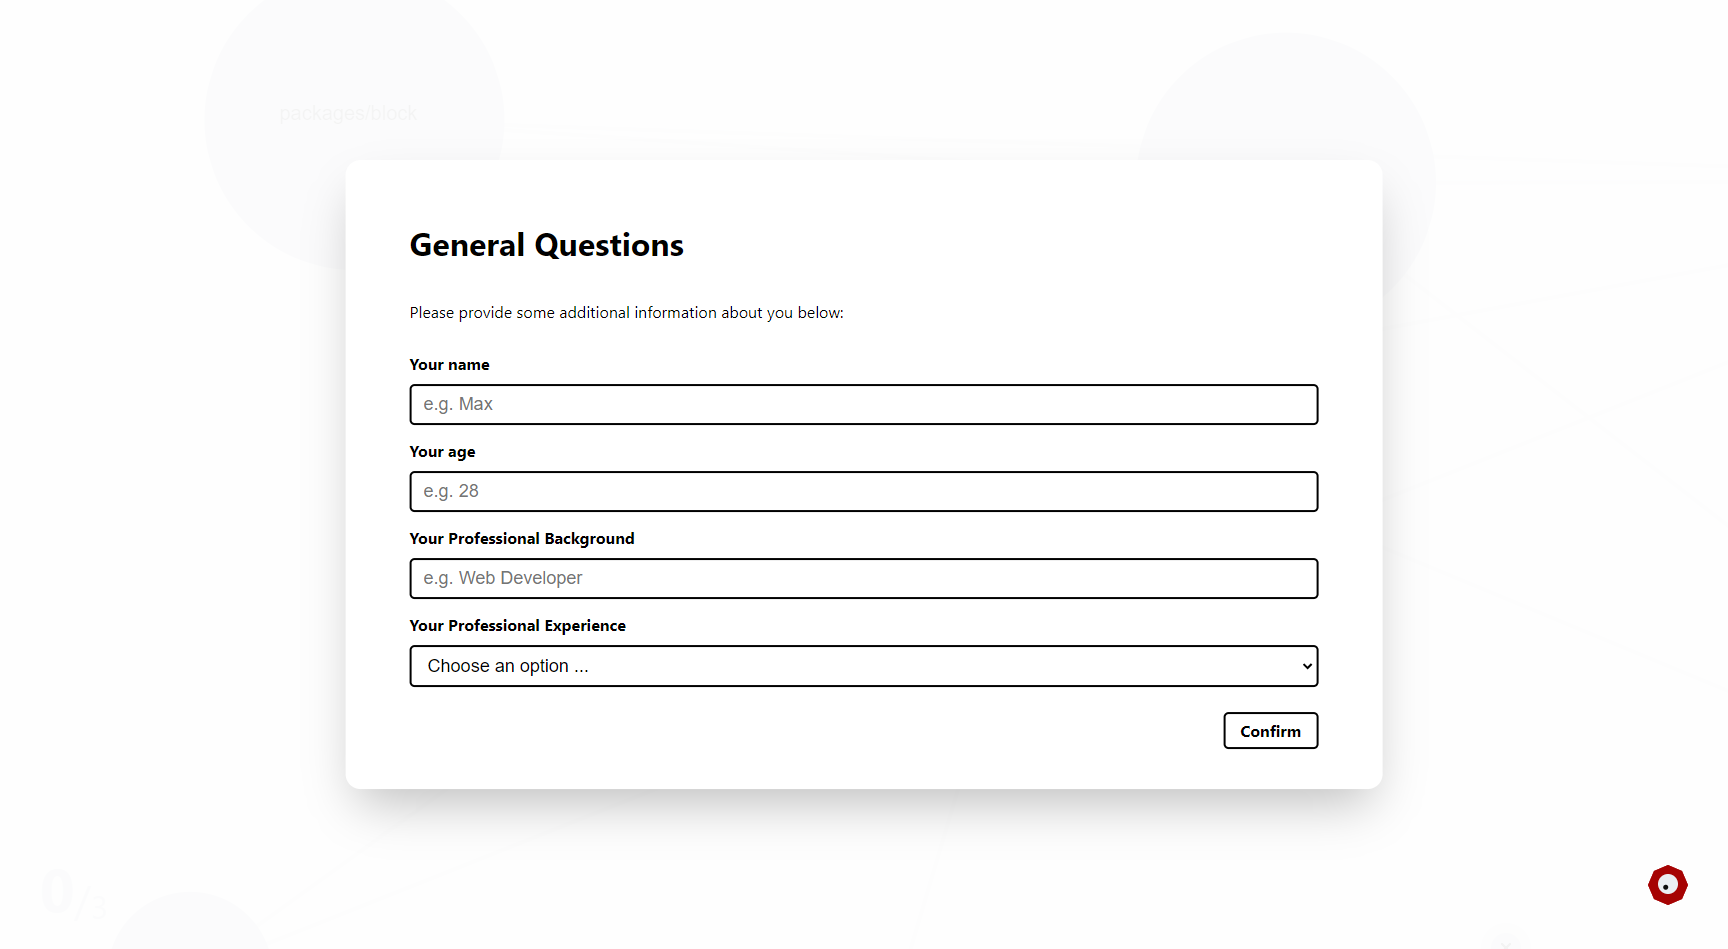
\includegraphics[width=\textwidth]{probesteps/step3.png}

  \subsection*{Step 4: Visualization Introduction}

  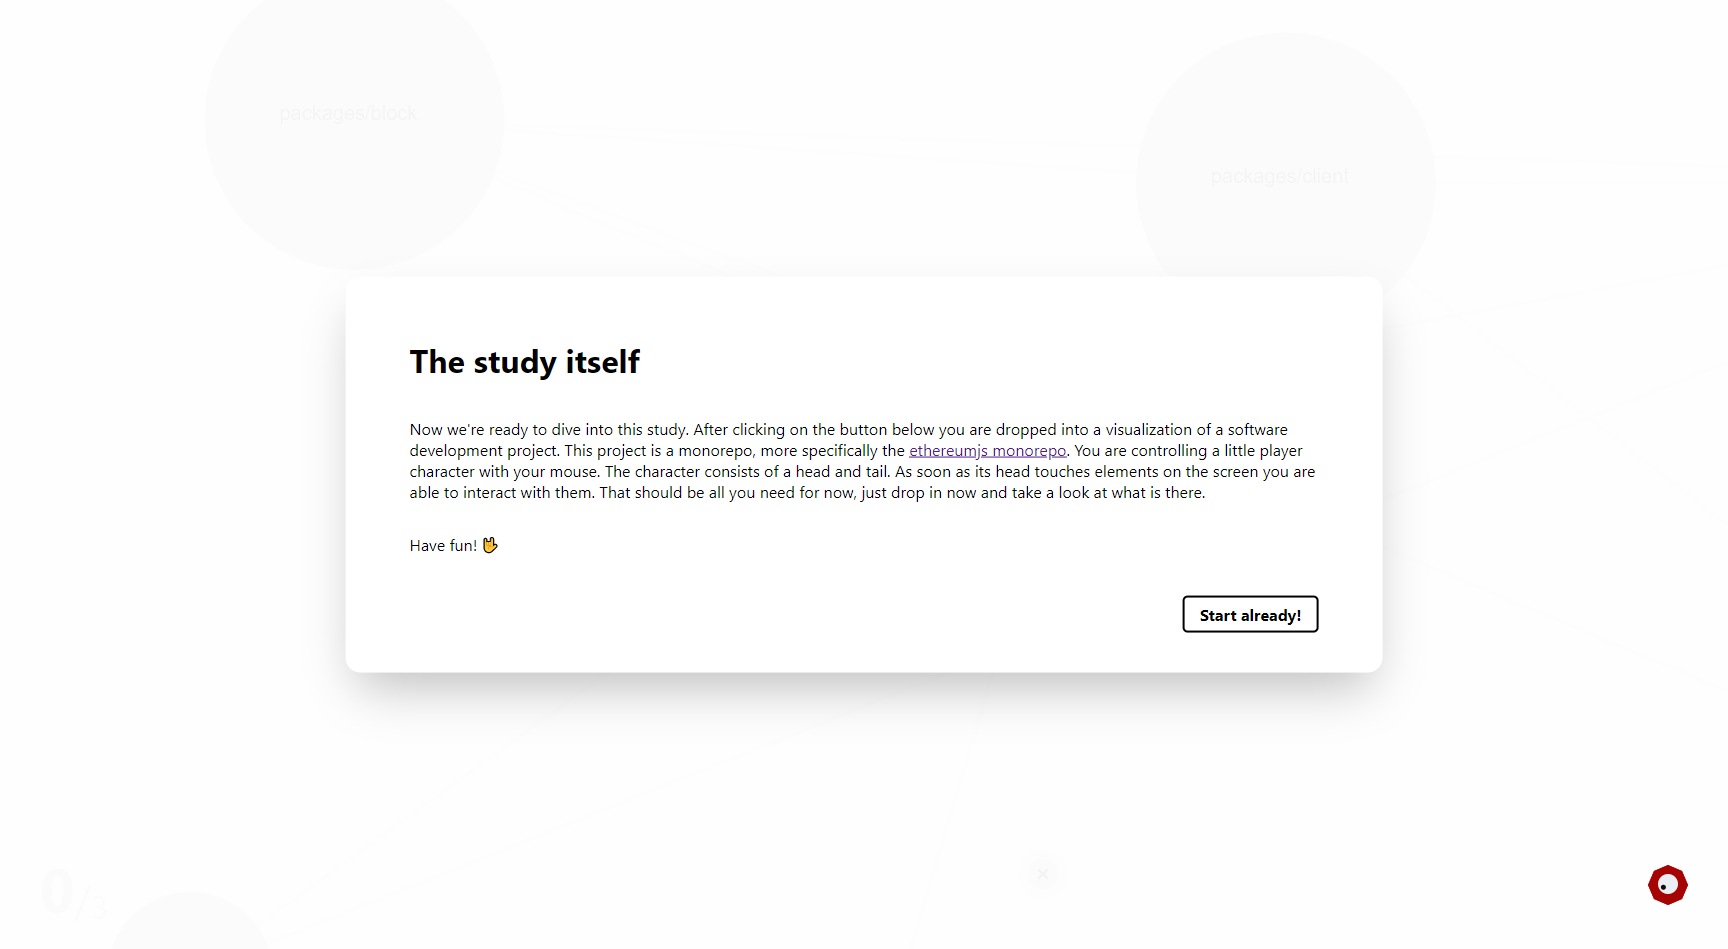
\includegraphics[width=\textwidth]{probesteps/step4.png}

  \subsection*{Step 5: Probe Overview Scene (Example)}

  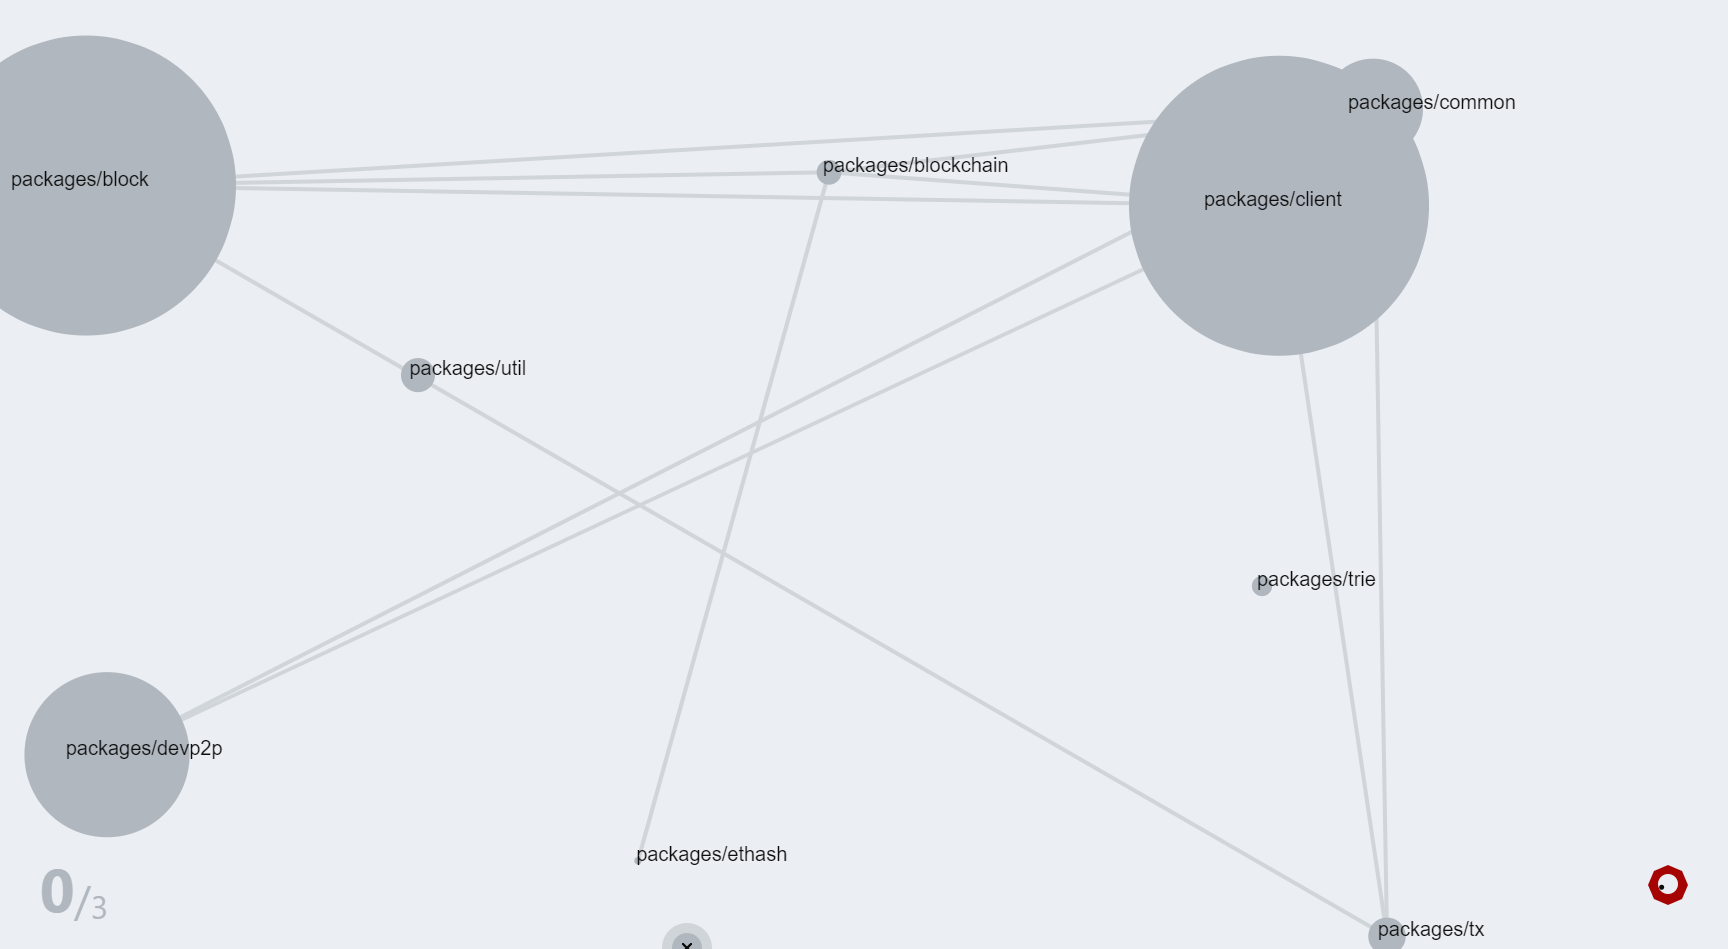
\includegraphics[width=\textwidth]{probesteps/step5.png}

  \subsection*{Step 6: Probe Detail Scene (Example)}

  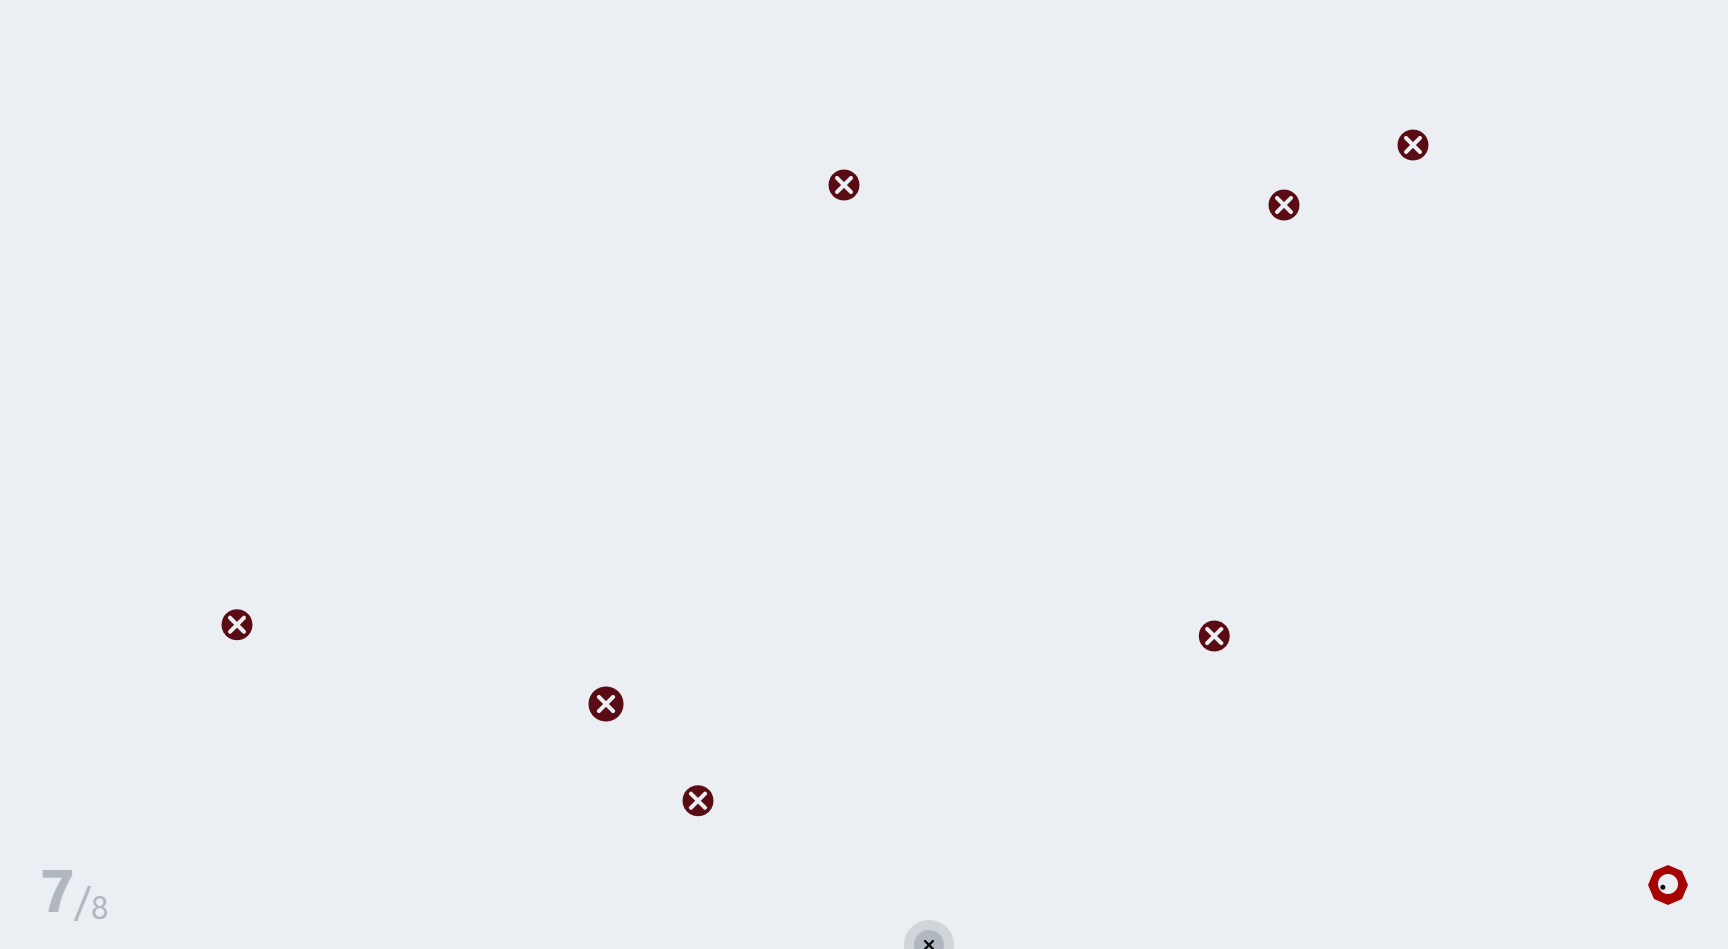
\includegraphics[width=\textwidth]{probesteps/step6.png}

  \subsection*{Step 7: Questions on the underlying project}

  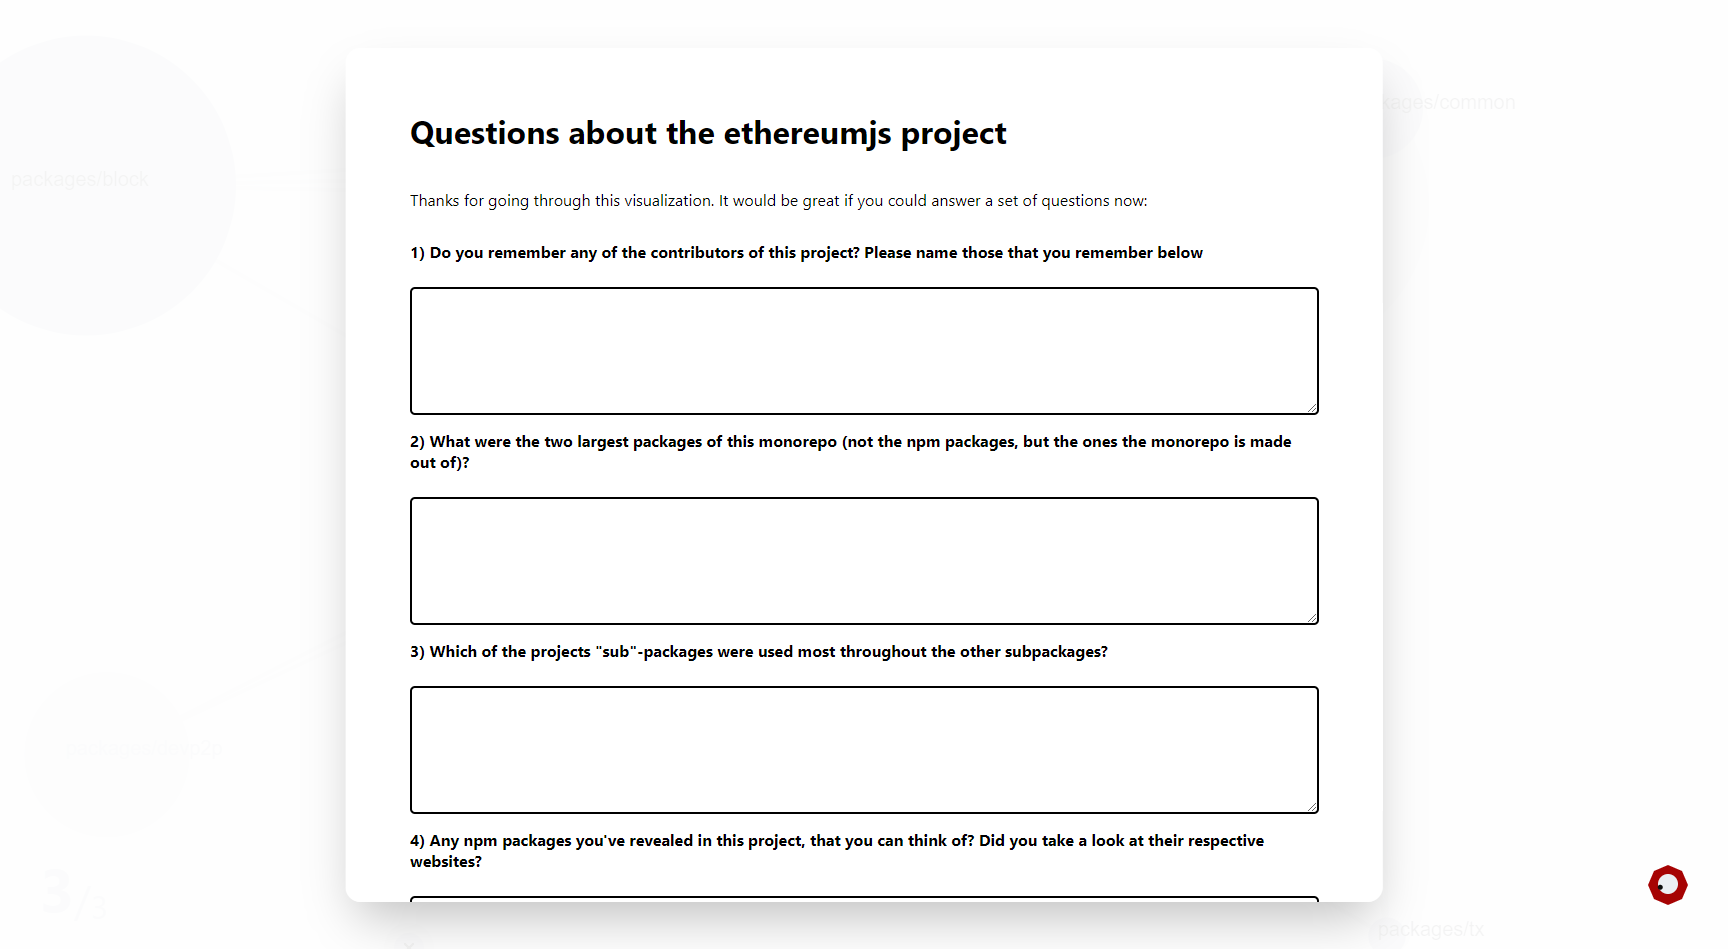
\includegraphics[width=\textwidth]{probesteps/step7.png}

  \subsection*{Step 8: Questions on the research topic}

  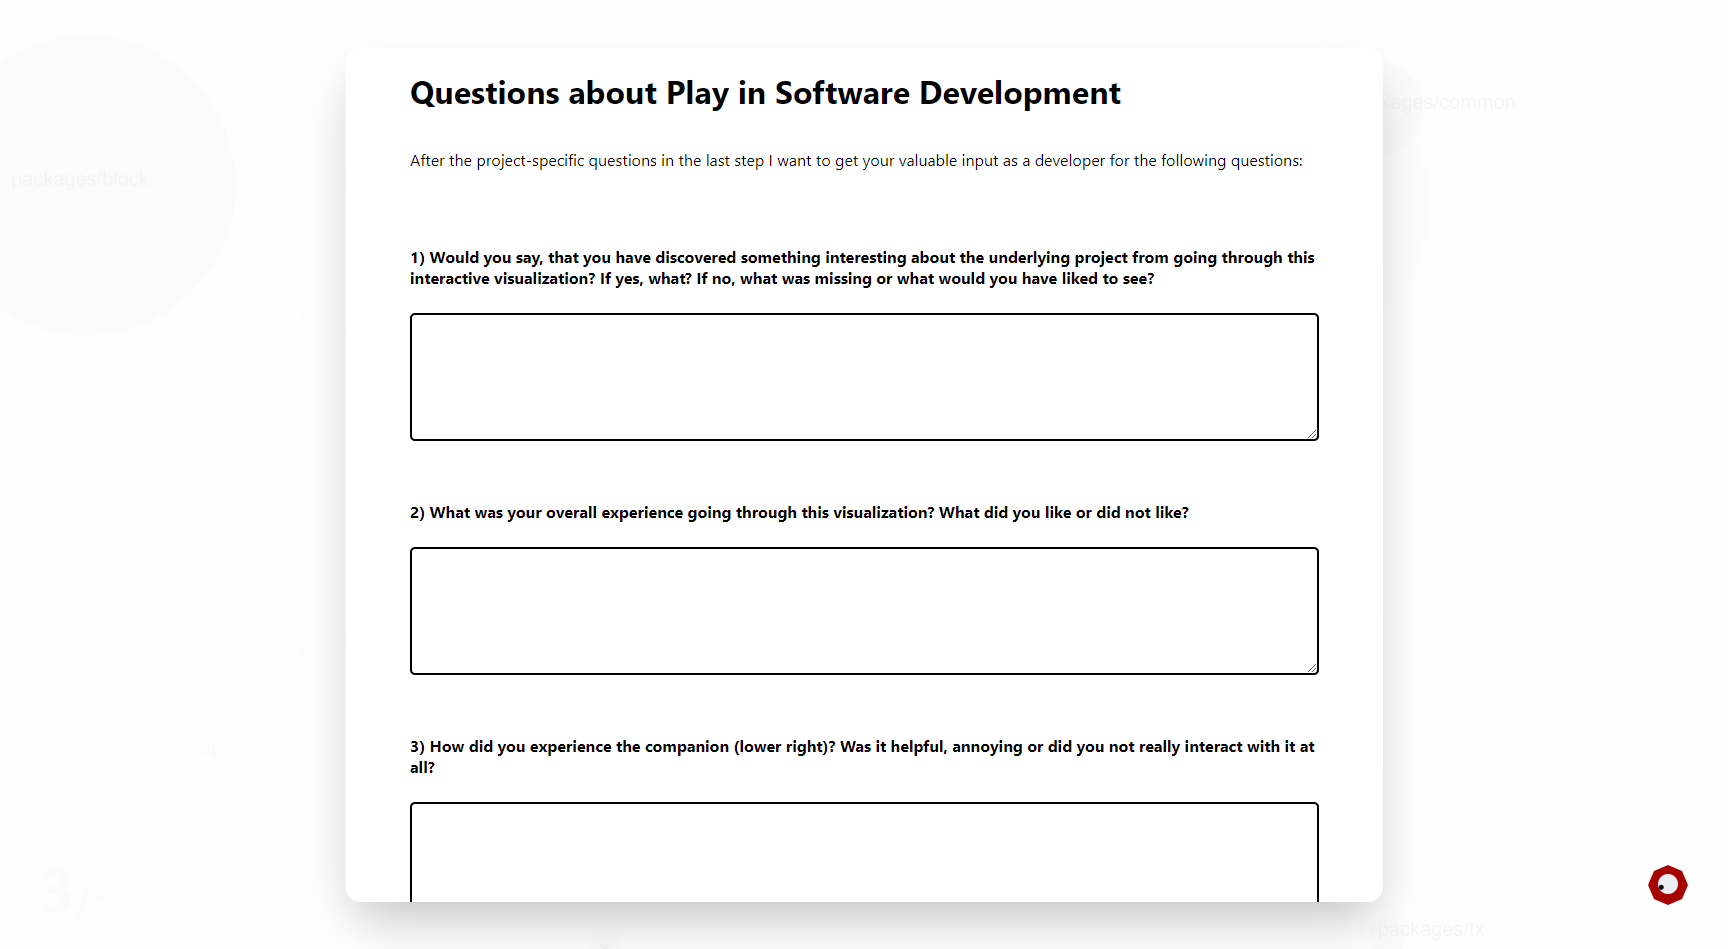
\includegraphics[width=\textwidth]{probesteps/step8.png}

  \subsection*{Step 9: Outro}

  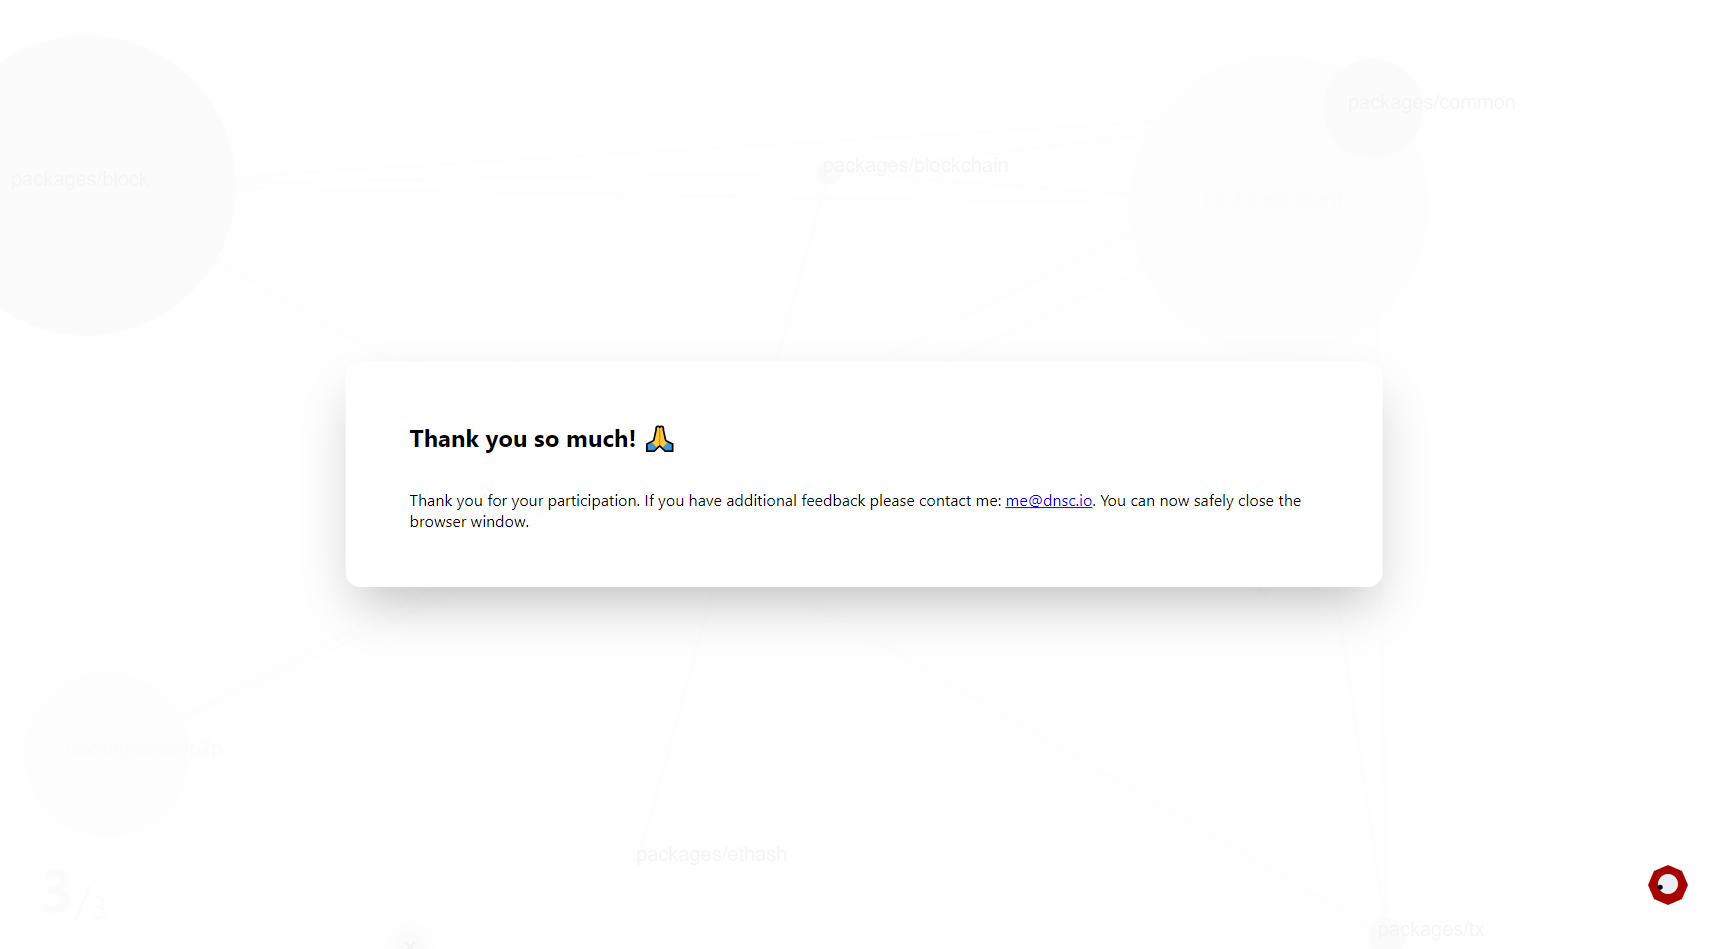
\includegraphics[width=\textwidth]{probesteps/step9.png}

  \newpage
  \section{Participants}
  \label{append:participants}

  \begin{table}[h]
    \begin{tabularx}{\textwidth}{|l|X|l|X|X|}
      \hline
      \textbf{Code} & \textbf{Name} & \textbf{Age} & \textbf{Professional Background} & \textbf{Professional Experience} \\ \hline \hline
      P1            & Anonymous     & 31           & Web Developer                    & 0-1 year                         \\ \hline
      P2            & Anonymous     & 28           & Full Stack Developer             & 1-3 years                        \\ \hline
      P3            & Jens          & 26           & Developer                        & 5-10 years                       \\ \hline
      P4            & Lukas         & 28           & Business Development             & 5-10 years                       \\ \hline
      P5            & Paolo Sfilio  & 28           & Software Developer               & 3-5 years                        \\ \hline
      P6            & Anonymous     & 36           & Backend Developer                & 10+ years                        \\ \hline
      P7            & Anonymous     & 28           & Data Scientist                   & 1-3 years                        \\ \hline
      P8            & Simon Hansen  & 27           & Web Developer                    & 3-5 years                        \\ \hline
      P9            & Anonymous     & 24           & .Net Dev                         & 3-5 years                        \\ \hline
    \end{tabularx}
  \end{table}


  \newpage
  \section{Aggregated Data from the Technology Probe Logs}
  \label{append:log-aggregated}

  Following are the general data points for each participant, aggregated from the raw logs of the technology probe. This text was generated programmatically, the respective script can be found within the accompanying repository at \texttt{./supplementary-material/data-analysis/aggregate-logs/aggregate-logs.js}.

  \subsection*{Participants}

  \subsubsection*{Participant P1}

  This participant spent a total time of \textbf{5 minutes 19 seconds} within the interactive part of the technology probe.

  During that time the participant clicked within the overview and to reveal (in the detail scenes) \textbf{119} times. The participant also tried to click the companion \textbf{8} times.


  \subsubsection*{Participant P2}

  This participant spent a total time of \textbf{6 minutes 49 seconds} within the interactive part of the technology probe.

  During that time the participant clicked within the overview and to reveal (in the detail scenes) \textbf{589} times. The participant also tried to click the companion \textbf{13} times.


  \subsubsection*{Participant P3}

  This participant spent a total time of \textbf{12 minutes 50 seconds} within the interactive part of the technology probe.

  During that time the participant clicked within the overview and to reveal (in the detail scenes) \textbf{224} times. The participant also tried to click the companion \textbf{10} times.


  \subsubsection*{Participant P4}

  This participant spent a total time of \textbf{3 minutes 15 seconds} within the interactive part of the technology probe.

  During that time the participant clicked within the overview and to reveal (in the detail scenes) \textbf{131} times. The participant also tried to click the companion \textbf{7} times.


  \subsubsection*{Participant P5}

  This participant spent a total time of \textbf{null [ed. note: not finished]} within the interactive part of the technology probe.

  During that time the participant clicked within the overview and to reveal (in the detail scenes) \textbf{40} times. The participant also tried to click the companion \textbf{0} times.


  \subsubsection*{Participant P6}

  This participant spent a total time of \textbf{2 minutes 18 seconds} within the interactive part of the technology probe.

  During that time the participant clicked within the overview and to reveal (in the detail scenes) \textbf{131} times. The participant also tried to click the companion \textbf{4} times.


  \subsubsection*{Participant P7}

  This participant spent a total time of \textbf{8 minutes 14 seconds} within the interactive part of the technology probe.

  During that time the participant clicked within the overview and to reveal (in the detail scenes) \textbf{561} times. The participant also tried to click the companion \textbf{45} times.


  \subsubsection*{Participant P8}

  This participant spent a total time of \textbf{9 minutes 50 seconds} within the interactive part of the technology probe.

  During that time the participant clicked within the overview and to reveal (in the detail scenes) \textbf{185} times. The participant also tried to click the companion \textbf{6} times.


  \subsubsection*{Participant P9}

  This participant spent a total time of \textbf{5 minutes 50 seconds} within the interactive part of the technology probe.

  During that time the participant clicked within the overview and to reveal (in the detail scenes) \textbf{184} times. The participant also tried to click the companion \textbf{6} times.



  \newpage
  \section{Qualitative Data -- Coding Units}
  \label{append:coding}

  On the following pages, the documented coding units for the qualitative content analysis can be found. These are the result of a multi-step process as described in chapter 5. The working document that includes every step of the process (Selection, Marking, Categories, Coding) can be accessed at the supplementary repository at the following path:

  \begin{center}
    \texttt{./supplementary-material/data-analysis/qualitative\_analysis.xslx}
  \end{center}

  \begin{landscape}
    \begin{longtable}{|p{0.8cm}|p{7cm}|p{3cm}|p{3cm}|p{5.5cm}|p{0.5cm}|}
      \hline
      \textbf{Part.} & \textbf{Marked Unit}                                                                                                                                                                                                                                                        & \textbf{Category Code}                   & \textbf{Contextual Unit (Feature)} & \textbf{Contextual Unit (Logs)}                                                                                                                    & \textbf{Nr.} \\ \hline
      \endhead
      %
      P1                   & didn't really care when I did this because I wasn't aware this was a thing                                                                                                                                                                                                  & Experience towards (playful) features    & Contributor Revealable             &                                                                                                                                                    & 1            \\ \hline
      P1                   & no emotional attachment to this project                                                                                                                                                                                                                                     & Contextual Considerations                &                                    &                                                                                                                                                    & 2            \\ \hline
      P1                   & Because contributors don't really help me to get started with a project I guess                                                                                                                                                                                             & Social Onboarding                        &                                    &                                                                                                                                                    & 3            \\ \hline
      P1                   & only had some 80 lines and I thought to myself 'well, that's not that big in my opinion'                                                                                                                                                                                    & Experience towards (playful) features    & Potential Issue Revealable         &                                                                                                                                                    & 4            \\ \hline
      P1                   & I didn't really get the impression of the existance of 'sub' packages, whatever they are supposed to be anyway                                                                                                                                                              & Experience towards (playful) features    & Overview Scene (Subpackages)       &                                                                                                                                                    & 5            \\ \hline
      P1                   & only check out npm packages when I actually have to work with them, not randomly only because they are used in a project                                                                                                                                                    & Technical Onboarding                     &                                    &                                                                                                                                                    & 6            \\ \hline
      P1                   & Not exactly sure what you mean with 'legacy' file                                                                                                                                                                                                                           & Experience towards (playful) features    & Potential Issue Revealable         &                                                                                                                                                    & 7            \\ \hline
      P1                   & actually interesting to get told about contributors and see their faces. Not that it would really help me getting into this project but yeah, gives it a more personal flavor                                                                                               & Social Onboarding                        &                                    &                                                                                                                                                    & 8            \\ \hline
      P1                   & during each discovery was still a bit big to digest in a playfull way I think                                                                                                                                                                                               & Attitude towards Playful elements        &                                    &                                                                                                                                                    & 9            \\ \hline
      P1                   & visualizations like images/icons rather than just plain text and a sample of the code and a link to the actual file                                                                                                                                                         & Improvements for implemented features    &                                    &                                                                                                                                                    & 10           \\ \hline
      P1                   & or an icon I learned earlier this represents a contributor                                                                                                                                                                                                                  & Improvements for implemented features    &                                    &                                                                                                                                                    & 11           \\ \hline
      P1                   & The texts where pretty repetitive and I stopped reading after 'contributor' so I might've missed any information that was unique to this slide                                                                                                                              & Experience towards (playful) features    &                                    &                                                                                                                                                    & 12           \\ \hline
      P1                   & I was a bit confused because I didn't know what to do when I reached the first blank slide                                                                                                                                                                                  & Experience towards (playful) features    &                                    & Can also be seen in the logs, No action at all in the beginning,  until companion message in both detail and overview scene (see logs lines 10-63) & 13           \\ \hline
      P1                   & helper on the bottom was quick to assist, though                                                                                                                                                                                                                            & Experience towards (playful) features    &                                    &                                                                                                                                                    & 14           \\ \hline
      P1                   & elements disappear, I would make them fade out rather than just getting invisible instantly                                                                                                                                                                                 & Improvements for implemented features    &                                    &                                                                                                                                                    & 15           \\ \hline
      P1                   & impression of revealing areas better when the initial background would be dark and when you trigger the sonar, everything inside the expanding circle is bright. Maybe with some something visual in the background that gives some depth perception.                       & Improvements for implemented features    &                                    &                                                                                                                                                    & 16           \\ \hline
      P1                   & came to help always at the right time. Good guy!                                                                                                                                                                                                                            & Experience towards (playful) features    &                                    & Both companion helping messages were shown, as seen in the logs (log lines 10, 60)                                                                 & 17           \\ \hline
      P1                   & To be honest, I don't really know. It strongly depends on the urgency to get familiar with a project I guess                                                                                                                                                                & Attitude towards Play in Onboarding      &                                    &                                                                                                                                                    & 18           \\ \hline
      P1                   & Exploring something like in this example can be frustrating if you really just want to get the gist of something because you stumble accross so many random things                                                                                                          & Attitude towards Play in Onboarding      &                                    &                                                                                                                                                    & 19           \\ \hline
      P1                   & this kind of visualization isn't the right thing to learn about a coding project. At least not for me.                                                                                                                                                                      & Attitude towards Play in Onboarding      &                                    &                                                                                                                                                    & 20           \\ \hline
      P1                   & hadn't had too much of these occations yet                                                                                                                                                                                                                                  & Organizational Onboarding                &                                    &                                                                                                                                                    & 21           \\ \hline
      P1                   & I set it up first to get a feeling for what I'm dealing with (if possible) and than I dig deeper into it                                                                                                                                                                    & Technical Onboarding                     &                                    &                                                                                                                                                    & 22           \\ \hline
      P1                   & I talk to those who set up or work on the project if possible                                                                                                                                                                                                               & Social Onboarding                        &                                    &                                                                                                                                                    & 23           \\ \hline
      P1                   & for my IDE, it's mostly stuff that helps visualize things like pairs of brackets and key words or variables vs functions and so on.                                                                                                                                         & Technical Onboarding                     &                                    &                                                                                                                                                    & 24           \\ \hline
      P1                   & I try to stick to conventions and write code that's hopefully easy to understand with meaningful variable and function names                                                                                                                                                & Technical Onboarding                     &                                    &                                                                                                                                                    & 25           \\ \hline
      P1                   & I'd provide some extra goals, like the first 5 questions about contributers I remember or not and so on so the explorer has something to aim for                                                                                                                            & Ideas on Playful Elements for Onboarding &                                    &                                                                                                                                                    & 26           \\ \hline
      P1                   & 'quests' can be aimed to point out core concepts of the project and guide the participant towards them.                                                                                                                                                                     & Ideas on Playful Elements for Onboarding &                                    &                                                                                                                                                    & 27           \\ \hline
      P1                   & Gamification is great to learn things like coding itself, like exploring a story with command line operations                                                                                                                                                               & Ideas on Playful Elements for Onboarding &                                    &                                                                                                                                                    & 28           \\ \hline
      P1                   & Exploring something in a playful way also needs to be done it each person's personal pace                                                                                                                                                                                   & Attitude towards Play in Onboarding      &                                    &                                                                                                                                                    & 29           \\ \hline
      P1                   & exploring something also needs time and is not fun if you are under preasure and you just want to get the gist of something                                                                                                                                                 & Attitude towards Play in Onboarding      &                                    &                                                                                                                                                    & 30           \\ \hline
      P1                   & As you did it in your example, I want to have the headspace to branch out and check out parts of the project that are maybe just nice to know but necessarely helping me with actually working on the project                                                               & Attitude towards Play in Onboarding      &                                    &                                                                                                                                                    & 31           \\ \hline
      P1                   & make the participants make solving problems, like searching for an answer for a specific question                                                                                                                                                                           & Ideas on Playful Elements for Onboarding &                                    &                                                                                                                                                    & 32           \\ \hline
      P1                   & let the participant choose a goal and give him or her some sort of quest line with a bunch of sub goals to achieve                                                                                                                                                          & Ideas on Playful Elements for Onboarding &                                    &                                                                                                                                                    & 33           \\ \hline
      P1                   & letting them to search for reusable components which are used throughout the project to make them aware they exist                                                                                                                                                          & Ideas on Onboarding Elements             &                                    &                                                                                                                                                    & 34           \\ \hline
      P1                   & what dependencies a main component has. Then you have just a portion of npm packages to digest                                                                                                                                                                              & Ideas on Onboarding Elements             &                                    &                                                                                                                                                    & 35           \\ \hline
      P1                   & Serve the project guided and bit by bit, only giving participants the choice what main goal they have or they want to achieve by playing this 'quest line'.                                                                                                                 & Ideas on Playful Elements for Onboarding &                                    &                                                                                                                                                    & 36           \\ \hline
      P3                   & Ich habe mir aber ein paar Profile angeguckt                                                                                                                                                                                                                                & Experience towards (playful) features    & Contributor Revealable             &                                                                                                                                                    & 37           \\ \hline
      P3                   & Anhang der Größe und Zeilenmenge hätte ich dem \textbackslash{}"refactor-worthy\textbackslash{}" aber in den meisten Fällen vermutlich zugestimmt.                                                                                                                          & Experience towards (playful) features    & Potential Issue Revealable         &                                                                                                                                                    & 38           \\ \hline
      P3                   & ungefähre Vorstellung davon bekommen, wie die Projekte untereinander zusammenhängen                                                                                                                                                                                         & Experience towards (playful) features    &                                    &                                                                                                                                                    & 39           \\ \hline
      P3                   & wenn ich es mir nicht merken konnte, war eine Visualisierung auf alle Fälle hilfreich                                                                                                                                                                                       & Experience towards (playful) features    &                                    &                                                                                                                                                    & 40           \\ \hline
      P3                   & schön durch die Vorstellung der Contributors ein paar Namen kennenzulernen, denen man im weiteren Verlauf des Projekt vermutlich häufiger über den Weg laufen wird                                                                                                          & Experience towards (playful) features    & Contributor Revealable             &                                                                                                                                                    & 41           \\ \hline
      P3                   & Mit der Vorstellung der großen \textbackslash{}"refactor-worthy\textbackslash{}" Dateien werden einem direkt mehrere Möglichkeiten eröffnet, in das Projekt einzusteigen                                                                                                    & Experience towards (playful) features    & Potential Issue Revealable         &                                                                                                                                                    & 42           \\ \hline
      P3                   & Mir fehlte ein wenig das fachliche über das Projekt. Was tut es? Wofür ist es gut? Nur anhand des Codes ist das schwierig zu verstehen.                                                                                                                                     & Improvements for implemented features    &                                    &                                                                                                                                                    & 43           \\ \hline
      P3                   & Im ersten Moment wusste ich nicht, wie ich starten sollte                                                                                                                                                                                                                   & Experience towards (playful) features    &                                    & As seen in the logs, companion messages appeared in both scenes (lines 9040, 9090)                                                                 & 44           \\ \hline
      P3                   & urch die Hilfen habe ich aber sehr schnell verstanden, wie der Ablauf gedacht ist                                                                                                                                                                                           & Experience towards (playful) features    &                                    & Both messages seen, after that clicking started as can be seen in logs (9040 and following, 9090 and following)                                    & 45           \\ \hline
      P3                   & Suchen der verschiedenen Punkte hat im ersten Moment Spaß gemacht, wurde anschließend aber ein bisschen nervig (vor allem weil einige Punkte vor einem abgehauen sind).                                                                                                     & Experience towards (playful) features    &                                    &                                                                                                                                                    & 46           \\ \hline
      P3                   & hilfreich um zu verstehen, wie das Onboarding zu bedienen ist                                                                                                                                                                                                               & Experience towards (playful) features    &                                    &                                                                                                                                                    & 47           \\ \hline
      P3                   & Leider sagt er nichts, wenn man auf ihn klick                                                                                                                                                                                                                               & Experience towards (playful) features    &                                    &                                                                                                                                                    & 48           \\ \hline
      P3                   & Wiederholung der Hilfe oder irgendein Feedback wären nett gewesen.                                                                                                                                                                                                          & Improvements for implemented features    &                                    &                                                                                                                                                    & 49           \\ \hline
      P3                   & ganz groben ersten Überblick über das Projekt zu verschaffen, würde ich so eine Visualisierung durchaus gut finden                                                                                                                                                          & Attitude towards Play in Onboarding      &                                    &                                                                                                                                                    & 50           \\ \hline
      P3                   & Wenn ich an einem neuen Projekt anfange, arbeite ich mich von außen immer weiter rein                                                                                                                                                                                       & Technical Onboarding                     &                                    &                                                                                                                                                    & 51           \\ \hline
      P3                   & Ablauf des Codes anhand von konkreten Interaktionen mit dem Programm                                                                                                                                                                                                        & Technical Onboarding                     &                                    &                                                                                                                                                    & 52           \\ \hline
      P3                   & Austausch mit erfahrenen Entwicklern finde ich dabei sehr wichtig                                                                                                                                                                                                           & Social Onboarding                        &                                    &                                                                                                                                                    & 53           \\ \hline
      P3                   & das durchgucken alter Issues und deren Lösungen finde ich immer sehr hilfreich                                                                                                                                                                                              & Organizational Onboarding                &                                    &                                                                                                                                                    & 54           \\ \hline
      P3                   & Entweder mir fällt selber ein Fehler/Verbesserung auf und ich möchte es umsetzen oder ich sehe Issues anderer Benutzer und möchte diese Lösen                                                                                                                               & Organizational Onboarding                &                                    &                                                                                                                                                    & 55           \\ \hline
      P3                   & versuche ich mich von oben nach unten durch den Code zu \textbackslash{}"wühlen\textbackslash{}" um irgendwann an der Stelle anzukommen, an der ich etwas ändern/verbessern möchte                                                                                          & Technical Onboarding                     &                                    &                                                                                                                                                    & 56           \\ \hline
      P3                   & verzweige ich oft in die verschiedenen Bereiche des Codes, die an dieser Stelle verwendet werden. So lerne ich nach und nach die Funktionen kennen und wie sie verwendet werden                                                                                             & Technical Onboarding                     &                                    &                                                                                                                                                    & 57           \\ \hline
      P3                   & Ich fände ein Beispiel-Issue spannend. Ein Fehlverhalten, das einem präsentiert wird und das man zu lösen hat. Das Beispiel-Issue sollte so gewählt sein, dass man an vielen wichtigen Stellen des Codes vorbeikommt                                                        & Ideas on Onboarding Elements             &                                    &                                                                                                                                                    & 58           \\ \hline
      P3                   & bevorzuge doch mehr den direkten Kontakt zu Kollegen/Contributors und das selbständige Entdecken des Codes.                                                                                                                                                                 & Social Onboarding                        &                                    &                                                                                                                                                    & 59           \\ \hline
      P3                   & Für den allerersten Überblick und eventuell einer fachlichen Vorstellung der Software finde ich spielerische Elemente durchaus angebracht                                                                                                                                   & Attitude towards Play in Onboarding      &                                    &                                                                                                                                                    & 60           \\ \hline
      P3                   & mehr bei den Open Source Projekten sehen, weil hier oft eine direkte und nahe Kommunikation mit anderen Entwicklern nur schwer möglich ist                                                                                                                                  & Contextual Considerations                &                                    &                                                                                                                                                    & 61           \\ \hline
      P3                   & Im Arbeitsumfeld sind Kollegen eher greifbar und bei Fragen ansprechbar                                                                                                                                                                                                     & Contextual Considerations                &                                    &                                                                                                                                                    & 62           \\ \hline
      P3                   & Vielleicht mit einem Art Wettbewerb wer einen gewissen Workflow schneller durchgespielt hat                                                                                                                                                                                 & Ideas on Playful Elements for Onboarding &                                    &                                                                                                                                                    & 63           \\ \hline
      P6                   & but many of the connections were overlapping, hard to see                                                                                                                                                                                                                   & Experience towards (playful) features    &                                    &                                                                                                                                                    & 64           \\ \hline
      P6                   & line/file size alone does not tell the whole story                                                                                                                                                                                                                          & Improvements for implemented features    &                                    &                                                                                                                                                    & 65           \\ \hline
      P6                   & Liked the connections and the overview map, helped me see at a glance what is in the project                                                                                                                                                                                & Experience towards (playful) features    &                                    &                                                                                                                                                    & 66           \\ \hline
      P6                   & missed actual textual content of the project besides the previews, maybe include more of the contents of the underyling project                                                                                                                                             & Improvements for implemented features    &                                    &                                                                                                                                                    & 67           \\ \hline
      P6                   & Liked the little worm character, felt smooth                                                                                                                                                                                                                                & Experience towards (playful) features    &                                    &                                                                                                                                                    & 68           \\ \hline
      P6                   & would have liked more connection to the source                                                                                                                                                                                                                              & Improvements for implemented features    &                                    &                                                                                                                                                    & 69           \\ \hline
      P6                   & Helpful as far as indicating what I have done                                                                                                                                                                                                                               & Experience towards (playful) features    & Companion                          &                                                                                                                                                    & 70           \\ \hline
      P6                   & not much interaction with it, could not click it besides messages                                                                                                                                                                                                           & Experience towards (playful) features    & Companion                          &                                                                                                                                                    & 71           \\ \hline
      P6                   & would like to see it on projects of another programming language\textbackslash{}nespecially those that maybe are not as cleanly divided into sub projects                                                                                                                   & Attitude towards Play in Onboarding      &                                    &                                                                                                                                                    & 72           \\ \hline
      P6                   & would have also liked to see more of the structure of the single sub projects                                                                                                                                                                                               & Improvements for implemented features    &                                    &                                                                                                                                                    & 73           \\ \hline
      P6                   & would probably still go at new projects in the IDE itself, seems more efficient at least for the source code                                                                                                                                                                & Attitude towards Play in Onboarding      &                                    &                                                                                                                                                    & 74           \\ \hline
      P6                   & I try to get access to everything that I need (git, deployment server, ...) and then set up the project locally and try to build it                                                                                                                                         & Technical Onboarding                     &                                    &                                                                                                                                                    & 75           \\ \hline
      P6                   & if there is at any point problems I try to contact the person who wrote the code otherwise the other team members already in the project                                                                                                                                    & Social Onboarding                        &                                    &                                                                                                                                                    & 76           \\ \hline
      P6                   & Best case there is documentation for the initial setup, but that is often missing                                                                                                                                                                                           & Organizational Onboarding                &                                    &                                                                                                                                                    & 77           \\ \hline
      P6                   & try to talk to project management to get to know the organizational structure                                                                                                                                                                                               & Organizational Onboarding                &                                    &                                                                                                                                                    & 78           \\ \hline
      P6                   & Navigation in code I do with IntelliJ and go-to-definition most of the time                                                                                                                                                                                                 & Technical Onboarding                     &                                    &                                                                                                                                                    & 79           \\ \hline
      P6                   & first step is always the documentation, if there are problems I google or search through the issue list of the package                                                                                                                                                      & Technical Onboarding                     &                                    &                                                                                                                                                    & 80           \\ \hline
      P6                   & For the source code, would have liked an approach that is near to the code, maybe within the IDE itself and more textual or a little helper within the IDE acting playful                                                                                                   & Improvements for implemented features    &                                    &                                                                                                                                                    & 81           \\ \hline
      P6                   & project organization structure maybe a clearer picture of who to talk to and communication with them as part of a game                                                                                                                                                      & Improvements for implemented features    &                                    &                                                                                                                                                    & 82           \\ \hline
      P6                   & do not think it can be efficient in day-to-day work                                                                                                                                                                                                                         & Attitude towards Play in Onboarding      &                                    &                                                                                                                                                    & 83           \\ \hline
      P6                   & maybe for looking at open source projects out of interests                                                                                                                                                                                                                  & Contextual Considerations                &                                    &                                                                                                                                                    & 84           \\ \hline
      P6                   & maybe for young developers or people starting with development                                                                                                                                                                                                              & Contextual Considerations                &                                    &                                                                                                                                                    & 85           \\ \hline
      P6                   & maybe include more of a progress status                                                                                                                                                                                                                                     & Improvements for implemented features    &                                    &                                                                                                                                                    & 86           \\ \hline
      P6                   & go all the way and create a 3D world from a project that you can go through, although that could be way too far from the project                                                                                                                                            & Ideas on Playful Elements for Onboarding &                                    &                                                                                                                                                    & 87           \\ \hline
      P8                   & Some code examples listed below looked to be refactor-worth. For example commented out console logs or very long config values mapped to string in inline calculations.                                                                                                     & Experience towards (playful) features    & Potential Issue Revealable         &                                                                                                                                                    & 88           \\ \hline
      P8                   & surprised that even a major project like ethereumjs has the same problems like many other projects like commented out code or console logs or very big util.ts files                                                                                                        & Technical Onboarding                     & Potential Issue Revealable         &                                                                                                                                                    & 89           \\ \hline
      P8                   & Some basic information like GitHub stars would be cool at the beginning                                                                                                                                                                                                     & Improvements for implemented features    &                                    &                                                                                                                                                    & 90           \\ \hline
      P8                   & I needed some time and the help box to understand, that I was supposed to click somewhere to reveal the information                                                                                                                                                         & Experience towards (playful) features    &                                    & Also can be seen in the logs, on the overview no help was shown, but then in detail scene it was (line 23471, companion message was closed)        & 91           \\ \hline
      P8                   & I had some problems catching the fast moving dots                                                                                                                                                                                                                           & Experience towards (playful) features    &                                    & Relatively long sequence of reveal clicks without clicking on an lement (e.g. json lines 23613-23755)                                              & 92           \\ \hline
      P8                   & That was fun at first, but at the end it was not that much fun anymore to catch the dots, because it was that easy                                                                                                                                                          & Experience towards (playful) features    &                                    &                                                                                                                                                    & 93           \\ \hline
      P8                   & visualisation of all modules looked a bit chaotic. At first I thought, \textbackslash{}"that should help me get a better overview?!\textbackslash{}"                                                                                                                        & Experience towards (playful) features    &                                    &                                                                                                                                                    & 94           \\ \hline
      P8                   & It came up when I was the first time in a sub module and didn't know what to do. There is was very helpful                                                                                                                                                                  & Experience towards (playful) features    & Companion                          & Can be seen on line 23471 - Companion was shown in submodule                                                                                       & 95           \\ \hline
      P8                   & I don't think that I would prefer such a game/interactive visualisation in contrast to just going throw the filestructure, because the game seemed to be a bit random                                                                                                       & Attitude towards Play in Onboarding      &                                    &                                                                                                                                                    & 96           \\ \hline
      P8                   & I don't know if the modules I checked out are the most important ones or not                                                                                                                                                                                                & Improvements for implemented features    &                                    &                                                                                                                                                    & 97           \\ \hline
      P8                   & usually it's a coworker introducing someone new to the project                                                                                                                                                                                                              & Social Onboarding                        &                                    &                                                                                                                                                    & 98           \\ \hline
      P8                   & I'm checking out a new github project, I just roam around and search for some modules and files whose name seem important to me                                                                                                                                             & Technical Onboarding                     &                                    &                                                                                                                                                    & 99           \\ \hline
      P8                   & I just go through the file structure in GitHub and when I wanna dig deeper I open the project in Intellj                                                                                                                                                                    & Technical Onboarding                     &                                    &                                                                                                                                                    & 100          \\ \hline
      P8                   & There could be some moving dots from module to module, depending on how often the module gets imported into another module                                                                                                                                                  & Improvements for implemented features    &                                    &                                                                                                                                                    & 101          \\ \hline
      P8                   & recognise which module is used a lot and which not that often                                                                                                                                                                                                               & Ideas on Onboarding Elements             &                                    &                                                                                                                                                    & 102          \\ \hline
      P8                   & some activity missing, many games have this discover, fight enemies concept                                                                                                                                                                                                 & Ideas on Playful Elements for Onboarding &                                    &                                                                                                                                                    & 103          \\ \hline
      P8                   & This guide is good for discovering                                                                                                                                                                                                                                          & Experience towards (playful) features    & Detail Scene (Within Subpackage)   &                                                                                                                                                    & 104          \\ \hline
      P8                   & some minigames like fighting the bugs or something similar could make it more interesting to play                                                                                                                                                                           & Ideas on Playful Elements for Onboarding &                                    &                                                                                                                                                    & 105          \\ \hline
      P8                   & some videos of the commit history of the project like                                                                                                                                                                                                                       & Ideas on Playful Elements for Onboarding &                                    &                                                                                                                                                    & 106          \\ \hline
      P8                   & In a work environment you are often applied to that project and there is someone who can introduce you                                                                                                                                                                      & Contextual Considerations                &                                    &                                                                                                                                                    & 107          \\ \hline
      P8                   & In open source project often someone new just joins randomly selfmotivated                                                                                                                                                                                                  & Contextual Considerations                &                                    &                                                                                                                                                    & 108          \\ \hline
      P8                   & playful automatic introduction brings more benefits for open source projects, than for work projects                                                                                                                                                                        & Contextual Considerations                &                                    &                                                                                                                                                    & 109          \\ \hline
      P8                   & find x items of y\textbackslash{}" feature (like the pigeons in gta4)                                                                                                                                                                                                       & Ideas on Playful Elements for Onboarding &                                    &                                                                                                                                                    & 110          \\ \hline
      P8                   & Some speaking character introducing with some basic information                                                                                                                                                                                                             & Ideas on Playful Elements for Onboarding &                                    &                                                                                                                                                    & 111          \\ \hline
      P8                   & Some character to follow, like a rabbit or something that you need to follow from module to module                                                                                                                                                                          & Ideas on Playful Elements for Onboarding &                                    &                                                                                                                                                    & 112          \\ \hline
      P8                   & area constraints, so that you discover a certain area, and after some tasks and knowladge gains you are allowed to discover a broader area                                                                                                                                  & Ideas on Playful Elements for Onboarding &                                    &                                                                                                                                                    & 113          \\ \hline
      P9                   & damit hab ich schon gearbeitet, hab aber nicht auf den link gklickt                                                                                                                                                                                                         & Experience towards (playful) features    & Package Revealable                 & went through pretty fast, not read too much in detail probably                                                                                     & 114          \\ \hline
      P9                   & grundsätzlich find ichs vertretbar, dass man bei über 1000 zeilen etwas refactoren sollte                                                                                                                                                                                   & Technical Onboarding                     & Potential Issue Revealable         &                                                                                                                                                    & 115          \\ \hline
      P9                   & übersicht gut, dass man alle packages auf einem platz sieht                                                                                                                                                                                                                 & Experience towards (playful) features    & Package Revealable                 &                                                                                                                                                    & 116          \\ \hline
      P9                   & mehr info zu den packages gewünscht, zusätzlich zu namen und größe, vielleicht direkt in der übersicht                                                                                                                                                                      & Improvements for implemented features    &                                    &                                                                                                                                                    & 117          \\ \hline
      P9                   & infos je package ganz gut, dass man die direkt die personen sieht mit dem was sie als letztes gemacht haben                                                                                                                                                                 & Experience towards (playful) features    & Package Revealable                 &                                                                                                                                                    & 118          \\ \hline
      P9                   & aufdecken war aber bisschen eintönig, da hätte mir was zusätzliches zu machen gefallen                                                                                                                                                                                      & Improvements for implemented features    &                                    &                                                                                                                                                    & 119          \\ \hline
      P9                   & fand die kleine animation mit dem auge ganz gut, aber viel interaktion gab es nicht                                                                                                                                                                                         & Experience towards (playful) features    & Companion                          &                                                                                                                                                    & 120          \\ \hline
      P9                   & gut bei neuen projekten grade bei größeren, wo es sonst schwierig is einen überblick zu bekommen\textbackslash{}nlinux-kernel würde mir einfallen, also bei großen ganz bekannten projekte, bei denen ich aber nicht unbedingt viel mit der programmiersprache gemacht habe & Contextual Considerations                &                                    &                                                                                                                                                    & 121          \\ \hline
      P9                   & klone mir das projekt als erstes und öffne es dann in meiner ide, da gehe ich dann vom main file ausgehend in die unterfiles, je nachdem was ich machen                                                                                                                     & Technical Onboarding                     &                                    &                                                                                                                                                    & 122          \\ \hline
      P9                   & in einer session zusammen die arbeit am projekt anzufangen um direkt einen ansprechpartner für fragen zu haben                                                                                                                                                              & Social Onboarding                        &                                    &                                                                                                                                                    & 123          \\ \hline
      P9                   & grade als einarbeitung in projekte, wo man schwierig einen überblick bekommen kann                                                                                                                                                                                          & Contextual Considerations                &                                    &                                                                                                                                                    & 124          \\ \hline
      P9                   & vielleicht nicht das schnellste, aber um sich spielerisch eine idee zu verschaffen eine gute idee                                                                                                                                                                           & Attitude towards Play in Onboarding      &                                    &                                                                                                                                                    & 125          \\ \hline
    \end{longtable}
  \end{landscape}
\end{appendices}
